\documentclass[10pt,twoside,openright]{memoir}
%\usepackage{createspace}
%\usepackage[size=pocket,noicc]{createspace}
\usepackage[paperwidth=8.5in, paperheight=11in,bindingoffset=.75in]{geometry}
%\usepackage[T1]{fontenc}
\usepackage[latin1]{inputenc}
\usepackage{tgtermes}
\usepackage{graphicx}
\usepackage{amssymb,mathtools}
%\usepackage{mathpazo}
\usepackage[protrusion=true,expansion=true]{microtype}
%\usepackage{type1cm}
%\usepackage{lettrine}

%\checkandfixthelayout

% See the ``Memoir customise'' template for some common customisations
% Don't forget to read the Memoir manual: memman.pdf

%\title{TITLE OF BOOK}
%\author{NAME OF AUTHOR}
%\date{} % Delete this line to display the current date
\usepackage{textcomp}
\usepackage{xcolor}
\usepackage{listings} % For code highlighting
\lstset{
  backgroundcolor=\color[rgb]{0.98,0.98,0.98},
  tabsize=4,
  rulecolor=,
  language=python,
        basicstyle=\scriptsize,
        upquote=true,
        aboveskip={1.5\baselineskip},
        columns=fixed,
        showstringspaces=false,
        extendedchars=true,
        breaklines=true,
        prebreak = \raisebox{0ex}[0ex][0ex]{\ensuremath{\hookleftarrow}},
        frame=single,
        showtabs=false,
        showspaces=false,
        showstringspaces=false,
        identifierstyle=\ttfamily,
        keywordstyle=\color[rgb]{0,0,1},
        commentstyle=\color[rgb]{0.133,0.545,0.133},
        stringstyle=\color[rgb]{0.627,0.126,0.941},
}

%% BEGIN TITLE

\makeatletter
\def\maketitle{%
  \null
  \thispagestyle{empty}%
  \vfill
  \begin{center}\leavevmode
    \normalfont
    {\LARGE\raggedleft \@author\par}%
    \hrulefill\par
    {\huge\raggedright \@title\par}%
    \vskip 1cm
%    {\Large \@date\par}%
  \end{center}%
  \vfill
  \null
  \cleardoublepage
  }
\makeatother
\author{NAME OF AUTHOR}
\author{Alan Lewis}
\title{Analytic Well Field Model Core Documentation}
\date{}

%%% BEGIN DOCUMENT

\begin{document}

\let\cleardoublepage\clearpage


\maketitle

\frontmatter

\null\vfill

\begin{flushleft}
\textit{NAME OF BOOK}


© COPYRIGHT INFO


ISBN--INFO

ISBN--13: 
\bigskip


ALL RIGHTS RESERVED OR COPYRIGHT LICENSE LANGUAGE

% ToC, etc
%%%\pagenumbering{roman}
\pagestyle{headings}
%%%%\pagestyle{Ruled}

\clearpage
\tableofcontents
\clearpage
\listoffigures
\clearpage
\listoftables


\end{flushleft}
\let\cleardoublepage\clearpage

\mainmatter
\sloppy


\chapter*{Introduction} % The asterisk leaves out this chapter from the table of contents

The Analytical Well Field Model (AWFM) is a collection of computer methods for processing
(and reducing) large amounts of pumping and water level data, running analytical models,
and providing meaningful estimates of aquifer and well-loss properties.

The core of AWFM provides many utilies for importing/exporting and processing data, but 
is unopinionated in that it makes it easy to add additional functionality when convenient.

With SCADA systems becoming more and more common, it is not unusual to see pumping and 
and water levels data sets containing hundreds-of-thousands or millions of records. While it is
advantageous to begin with such high-resolution data, it is largely redundant. 

\mainmatter

%----------------------------------------------------------------------------------------
% CHAPTER MATHEMATICAL BASIS
%----------------------------------------------------------------------------------------

\chapter{Mathematical Basis}

\section{Forward Model}
About forward model

\section{Inverse Model}
About inverse model


%----------------------------------------------------------------------------------------
% CHAPTER Installation
%----------------------------------------------------------------------------------------

\chapter{Installation}

\section{Linux}
\section{Windows}
\section{Apple}

%----------------------------------------------------------------------------------------
% CHAPTER Timeseries
%----------------------------------------------------------------------------------------

\chapter{Timeseries Class}

The Timeseries class stores and processes arrays of time-value pairs. Examples of
Timeseries objects include pumping rates and water levels.

\section{Instantiating and Building Timeseries Object}

The \textbf{Timeseries} class lives inside the \emph{awfm.core} module. It is 
instantiated with no arguments and initially contains no data. The timeseries
is populated with data using the \emph{append} function, which takes two arguments: 
a time and an associated value. 

\begin{figure}[!h]
\begin{lstlisting}[language=python]
from awfm.core import Timeseries

ts = Timeseries()
ts.append(0, 10) # time = 0, value = 10
ts.append(1, 20)
ts.append(2, 30)
\end{lstlisting}
\caption{Example of creating and populating a Timeseries instance}
\end{figure}

An important feature of the \emph{append} method is that time-value pairs
must be inserted in chronological order. If an attempt is made to insert a 
time-value pair that is out of order, the pair will not be appended to the
timeseries, and an error will be logged. Every function 
that acts on a timeseries assumes that data is stored in chronological order.

\begin{figure}[!h]
\begin{lstlisting}[language=python]
from awfm.core import Timeseries

ts = Timeseries()
ts.append(0, 10)
ts.append(2, 30)
ts.append(1, 20)

if ts.errors:
    print(errors)
    exit(0)
\end{lstlisting}
\caption{How to check that a timeseries has been populated correctly}
\end{figure}

\section{Timeseries Methods}

There are several useful methods that can be performed on a \textbf{Timeseries}
instance. None of the methods described here will modify a timeseries instance.
Rather, a modified timeseries will be returned. 

\subsection{zero\_below\_magnitude}

\emph{zero\_below\_magnitude} is a method that converts all values in a timeseries
below some given magnitude to zero. This method is useful for cleaning
out noise in pumping rate data. It is common for SCADA systems to continue
collecting pumping rate data at some small magnitude after the system
has been turned off. For modeling purposes, one may want to simply consider
these values to be 0. 

\begin{figure}[!h]
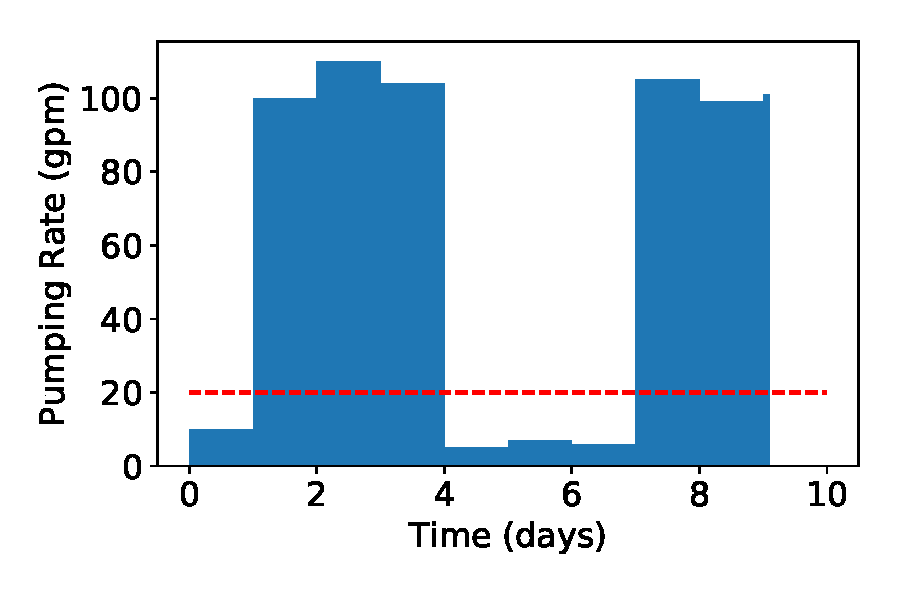
\includegraphics[width=7cm]{python/timeseries_zero_below_magnitude_before.pdf}
\hspace{\fill}
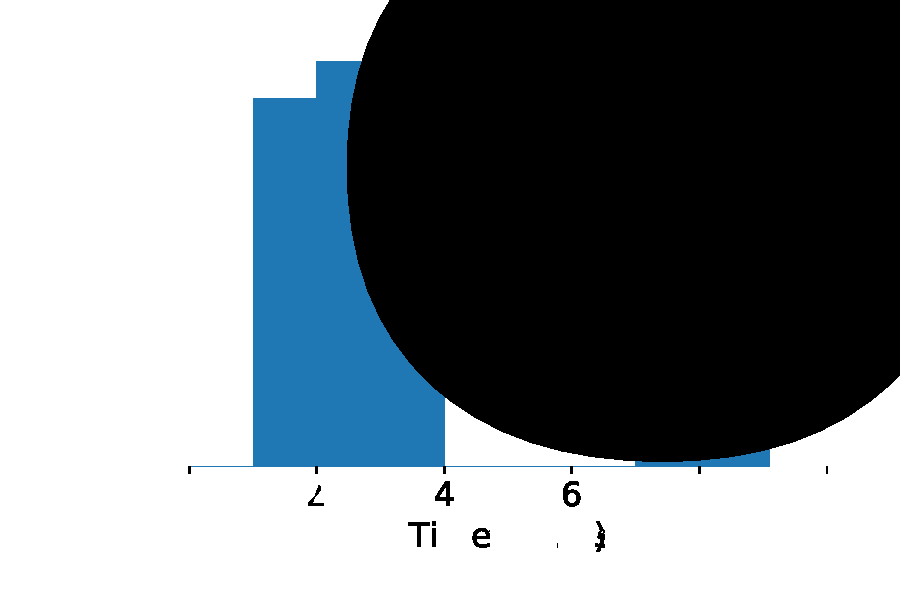
\includegraphics[width=7cm]{python/timeseries_zero_below_magnitude_after.pdf}
\caption{ \emph{zero\_below\_magnitude} example plots. 
    Original timeseries (left) is modified (right) using a threshold of 20 gpm.}
\end{figure}

\begin{figure}[!h]
\begin{lstlisting}[language=python]
ts = Timeseries()
# ... Timeseries is populated here

ts_modified = ts.zero_below_magnitude(20)
\end{lstlisting}
\caption{Example usage of \emph{zero\_below\_magnitude}}
\end{figure}

\subsection{consolidate\_adjacent\_equal\_values}
\emph{consolidate\_adjacent\_equal\_values} is an important method for reducing
the size of a data set. Many aquifer drawdown models, such as the Theis solution, 
only require \emph{changes} in pumping rates as model inputs. If the pumping rate
at a well stays constant for a long period of time, the data recorded may be largely
redundant. \emph{consolidate\_adjacent\_equal\_values} filters a timeseries
such that only changes are kept. 

\begin{figure}[!h]
\begin{tabular}{c c}
    \hline
    Time & Q \\ \hline
    0 & 120.0 \\
    1 & 120.0 \\
    2 & 118.0 \\
    3 & 0 \\
    4 & 0 \\
    5 & 0 \\
    6 & 0 \\
    7 & 112.0 \\
    8 & 110.0
\end{tabular}
\hspace{5cm} 
\begin{tabular}{c c}
    \hline
    Time & Q \\ \hline
    0 & 120.0 \\
    2 & 118.0 \\
    3 & 0 \\
    7 & 112.0 \\
    8 & 110.0
\end{tabular}
\caption{Original timeseries (left) reduced by 
\emph{consolidate\_adjacent\_equal\_values}} (right)
\end{figure}

\emph{consolidate\_adjacent\_equal\_values} works best when used immediately
after \emph{zero\_below\_magnitude} and/or \emph{round\_to\_nearest} methods.

\subsection{round\_to\_nearest}
\emph{round\_to\_nearest} rounds each value in a timeseries to some nearest
magnitude given as the method argument, using the following function:

% rounded_value = round(self.vs[i]/v)*v
$$v_{rounded} = \textrm{round}(\frac{v}{v_{magnitude}})*v_{magnitude}$$

For example, given a value ($v$) of $118.0$, rounded to the nearest 
($v_{magnitude}$) 10:

$$v_{rounded} = \textrm{round}\Big(\frac{118.0}{10}\Big)*10$$
$$v_{rounded} = \textrm{round}(11.8)*10$$
$$v_{rounded} = 12*10$$
$$v_{rounded} = 120$$

\begin{figure}[!h]
\begin{tabular}{c c}
    \hline
    Time & Q \\ \hline
    0 & 120.0 \\
    1 & 120.0 \\
    2 & 118.0 \\
    3 & 0 \\
    4 & 0 \\
    5 & 0 \\
    6 & 0 \\
    7 & 112.0 \\
    8 & 110.0
\end{tabular}
\hspace{2cm} 
\begin{tabular}{c c}
    \hline
    Time & Q \\ \hline
    0 & 120.0 \\
    1 & 120.0 \\
    2 & 120.0 \\
    3 & 0 \\
    4 & 0 \\
    5 & 0 \\
    6 & 0 \\
    7 & 110.0 \\
    8 & 110.0
\end{tabular}
\hspace{2cm} 
\begin{tabular}{c c}
    \hline
    Time & Q \\ \hline
    0 & 120.0 \\
    3 & 0 \\
    7 & 110.0
\end{tabular}
\caption{Original timeseries (left) rounded to the nearest 10
(middle) using \emph{round\_to\_nearest} and then being
reduced using \emph{consolidate\_adjacent\_equal\_values}} (right)
\label{fig:roundedandreduced}
\end{figure}

\begin{figure}[!h]
\begin{lstlisting}[language=python]
ts = Timeseries()
# ... Timeseries is populated here

ts_modified = ts.round_to_nearest(10).consolidate_adjacent_equal_values()
\end{lstlisting}
\caption{Example method calls used to calculate values in Figure \ref{fig:roundedandreduced}}
\end{figure}

\subsection{average\_by\_sign}
\emph{average\_by\_sign} averages timeseries data by sign, where sign is:

\begin{equation}
  sign = 
    \begin{cases}
      1 & \text{if $v > 0 $} \\
      0 & \text{if $v = 0 $} \\
     -1 & \text{if $v < 0 $} 
    \end{cases}
\end{equation}

In terms of well production, sign$=1$ would mean groundwater extraction, 
sign$=-1$ would mean groundwater injection, and sign$=0$ would mean that
there is no activity.

 \emph{average\_by\_sign} might be the simplest way to quickly reduce a 
 data set by (potentially) several orders of magnitude.

\end{document}